\documentclass[10pt,letterpaper]{article}
\usepackage[dvipsnames]{xcolor}
\usepackage{outlines}
\usepackage{amsmath}
\usepackage{tikz}
\usepackage{hyperref}
\usepackage{enumitem}
\usepackage{cancel}
\usepackage{subcaption}
\DeclareCaptionOptionNoValue{centering}{\centering} % Make sure everything is centered in subs
\captionsetup[sub]{centering}

\usepackage{algorithm}
\usepackage[noend]{algpseudocode}
\makeatletter
\def\BState{\State\hskip-\ALG@thistlm}
\makeatother

\usepackage{multirow}
\usepackage{cancel}
\usepackage{float}

\usepackage{parskip}

\usepackage{slantsc,lmodern}

\usepackage{pgfplotstable,booktabs}
\usepackage{framed}
\definecolor{shadecolor}{rgb}{0.9,0.9,0.9}

\usepackage{gensymb}

\usepackage{paralist}

\usepackage[paper=a4paper,margin=1in]{geometry}

\usepackage{etoolbox}

\newcommand{\volume}{{\ooalign{\hfil$V$\hfil\cr\kern0.08em--\hfil\cr}}}

\makeatletter
\g@addto@macro\@floatboxreset\centering
\makeatother

\author{Thaddeus Hughes \\ hughes.thad@gmail.com \\ thaddeus-maximus.github.io}
\date{\today}
\title{Documentation and Validation of EveryCalc's Transmission Strength Tool}

\begin{document}
	\maketitle
	
	\begin{abstract}
		Making sure a gearbox is designed to handle the stresses that are inflicted upon it can be a tedious and repetative task, but is rather formulaic, making it an excellent candidate for an automated tool with a flexible frontend.
	\end{abstract}
	
\section{Strength of Gears}
	There are many failure points on a gear, but the most common and the only one that can be fairly analyzed without knowing the exact geometry (such as pocketing, shaft interface geometry) is that of the gear tooth.
	\href{https://www.engineersedge.com/gears/gear-tooth-strength.htm}{\underline{Engineer's Edge}} explains the common way of calculating tooth strength by considering the load as being fully transmitted by one tooth which is a beam in bending.

	\begin{align}
		W_t = \frac{S w Y(N,\alpha)}{D_p}, 
	\end{align}

	where $W_t$ is the maximum allowable tangential force on the gear tooth, $S$ is the maximum allowable stress in the gear, $w$ is the width of the tooth, $Y$ is the \textit{Lewis Factor}, and $D_{p}$ is the diametral pitch (not the module, which is the reciprocal of the diametral pitch).

	To determine the torque-carrying capacity of the gear, we substitute in an expression for torque $T$,

	\begin{align}
		T = W_t \ r &= W_t \frac{N}{2 \ D_p} \\
		\frac{2 \ D_p}{N} \ T &= \frac{S \ w \ Y(N,\alpha)}{D_p} \\
		T_{max, gear} &= \frac{S_{gear} \ w \ Y(N,\alpha) \ N}{2 \ D_p^2}
	\end{align}

	The Lewis Factor $Y$ is obtained by 1-D interpolation.

	\begin{figure}[H]
		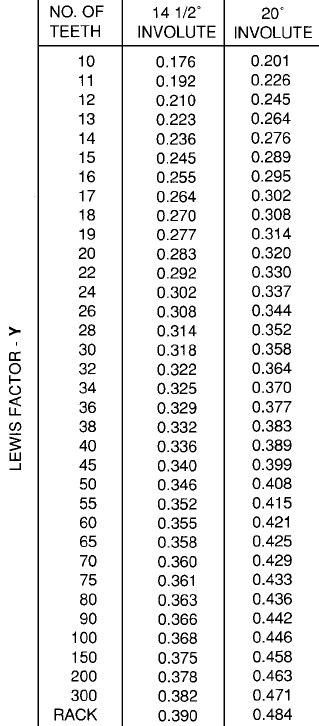
\includegraphics[width=0.5\textwidth]{lewis_factor_table.png}
		\caption{Lewis Factor values, tabulated}
	\end{figure}

	$S_{gear}$ will be considered to be the tensile yield strength.

	\textit{Observations: to make a gear stronger, increasing its width or base material strength will have a linear benefit. Increasing the number of teeth will have a hyperlinear benefit (as it influences the lewis factor). Using a lower pressure angle will help the lewis factor. Using a lower diametral pitch (a coarser gear) will also improve strength.}

\section{Strength of Shafts}
	Shafts are considered to be in pure torsion. This means that they experience stress that can be computed as
	\begin{align}
		\sigma_{shear,outside} = \frac{T r}{J} = \frac{T d}{2 J}
	\end{align}

	Solving for the torque and substituting in maximum allowable shear stress $S_{shaft}$ for $\sigma$ yields
	\begin{align}
		T_{max,shaft} = S_{shaft} \frac{J}{r}
	\end{align}
	$S_{shaft}$ will be the maximum shear stress, or the tensile yield stress divided by two.

\section{Strength of Timing Belt Runs}
	Belt strength is calculated from the tables in the \href{https://www.gates.com/content/dam/gates/home/resources/resource-library/catalogs/light-power-and-precision-manual.pdf}{\underline{Gates Light Power and Precision Manual}}.

	\begin{figure}[H]
	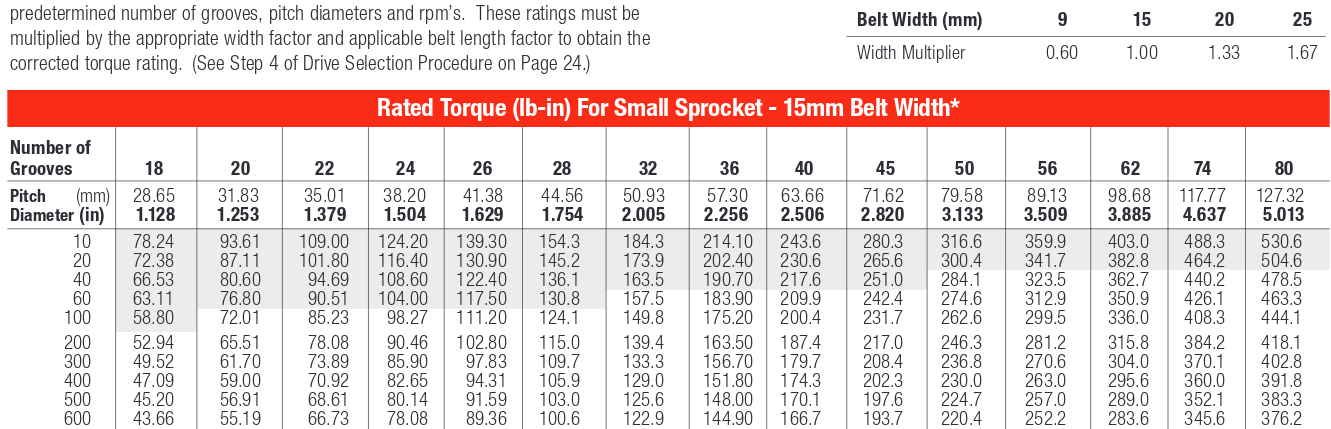
\includegraphics[width=\textwidth]{beltrating_a.png}
	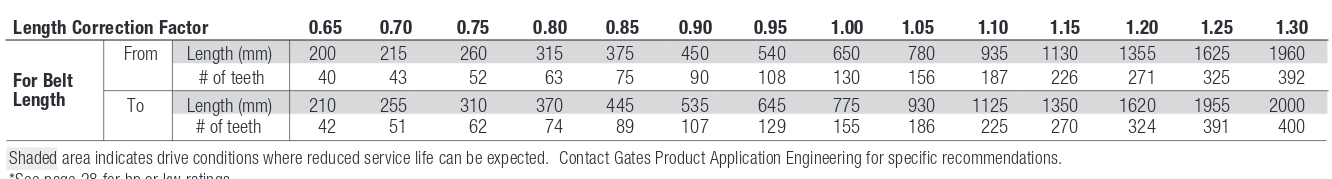
\includegraphics[width=\textwidth]{beltrating_b.png}
	\caption{Exemplary data from the Gates manual.}
	\end{figure}

	These tables list allowable pulley torque $T(\omega, N)$ as a function of RPM $\omega$ and pulley teeth $N$. Note that 6 teeth should be in engagement.
	2-D interpolation is used to determine values on the in-betweens.
	Tabulated values outside the bounds are extrapolated. Omitted values are presumed to be zero.

	\begin{align}
		T_{base} &= \text{interp2D}(\{N\}, \{\omega\}, [T], N_{sprocket}, \omega_{sprocket}) \\
		K_{length} &= \text{interp1D}(\{L\}, \{K_{lengths}\}, \{L_{belt}\}) \\
		K_{width} &= \text{lookup}(\{w\}, \{K_{widths}\}, \{w_{belt}\}) \\
		T_{rated,\ sprocket} &= K_{length} \times K_{width} \times T_{base}
	\end{align}

	It should also be noted that the number of teeth engaged with the pulley is recommended to be no less than 6.

\section{Strength of COTS Planetaries}
	\subsection{VexPro VersaPlanetary}
	\href{https://www.vexrobotics.com/versaplanetary.html}{\underline{VexPro's VersaPlanetaries}} come with a \href{https://docs.google.com/gview?url=http://link.vex.com/vexpro/pdf/VersaPlanetary-LoadRatings}{\underline{Load Rating Guide}}.

	The key failure points identified are:
	\begin{asparaitem}
		\item 10:1, 9:1, and 7:1 stages have a torque capacity of \textbf{100 N-m}.
		\item Ratchet slices have a torque capacity of \textbf{160 N-m}.
		\item 1/2" hex output shafts fail at \textbf{157 N-m}.
		\item 1/2" round output shafts fail at \textbf{130 N-m}.
		\item 3/8" hex output shafts fail at \textbf{57 N-m}.
		\item CIM-style output shafts fail at \textbf{29 N-m}.
	\end{asparaitem}

	These ratings, as this calculator, do not take into consideration bending loads which could further derate the carrying capacity.

	\subsection{AndyMark 57 Sport}
	\href{https://www.andymark.com/products/57-sport-options}{\underline{AndyMark's 57 Sport Gearboxes}} are rated on a per-gearbox configuration with a maximum torque capacity.

	\subsection{REV UltraPlanetary}
	\href{https://www.revrobotics.com/rev-41-1600/}{\underline{REV's UltraPlanetaries}} have a load rating of 40 N-m at the final cartridge (output).
	
\end{document}